\documentclass[sigconf,nonacm]{acmart}

\title{Evolutionary LLMs for Automated Coordination Algorithm Design in System-Level Architectures}

\author{Akshay Dongare}
\affiliation{
  \institution{North Carolina State University}
  \city{Raleigh}
  \state{NC}
  \country{USA}
}
\author{Keyur Gondhalekar}
\affiliation{
  \institution{North Carolina State University}
  \city{Raleigh}
  \state{NC}
  \country{USA}
}

\begin{document}

\begin{abstract}
Modern software systems rely on complex coordination logic across interacting components, yet such logic is often manually designed, brittle, and difficult to optimize. This paper explores whether large language models (LLMs), embedded within evolutionary frameworks, can automatically generate and improve active-learning configuration heuristics for system-level architectures. We conduct a structured literature analysis to identify gaps in current research, revealing a lack of work at the intersection of evolutionary search, algorithm generation, and system-level optimization. To investigate this gap, we evaluate the HSEvo evolutionary LLM framework on the MOOT (Multi-Objective Optimization Tasks) benchmark. Our results demonstrate that LLM-driven evolutionary approaches can generate effective heuristics, outperforming static baselines on the MOOT benchmark. We discuss trade-offs in cost, interpretability, and solution diversity, and outline explicit threats to validity and directions for future work.
\end{abstract}

\maketitle

\section{Introduction}

Modern software engineering is characterized by complex systems composed of interacting components such as multi-agent LLM workflows and cloud microservices. These systems require coordination logic that determines how components interact, route tasks, and allocate resources. While flexible architectures allow many design choices, they introduce a large space of algorithmic parameters and routing heuristics that must be tuned.

Hand-crafted coordination logic is often poorly documented, difficult to scale, and prone to subtle interactions. As systems grow in complexity, manual tuning becomes infeasible and unreliable. Therefore, static coordination algorithms become a liability without adaptive tool support.

Recent work has explored the use of large language models (LLMs) for optimization tasks \cite{romera2023mathematical}. However, most approaches focus on generating solutions or tuning parameters rather than evolving the underlying algorithms themselves. This paper explores whether LLMs embedded within evolutionary frameworks can generate and optimize coordination strategies across real-world software engineering optimization tasks.

To ensure realism and generalizability, we evaluate our approach using the MOOT (Multi-Objective Optimization Tasks) repository, which provides a diverse set of multi-objective optimization problems derived from software engineering contexts.

\section{Research Questions}

\textbf{RQ1:} Can an LLM embedded within an evolutionary framework automatically generate and evolve superior configuration heuristics for system-level architectures compared to static heuristic baselines?

\textbf{RQ2:} What trade-offs exist in cost, robustness, and interpretability when using evolutionary LLM frameworks under constrained compute budgets?

\section{Contributions}

This paper makes the following contributions:
\begin{itemize}
\item Proposes a framework using evolutionary LLMs to generate coordination algorithms for system-level architectures.
\item Provides an empirical comparison between LLM-generated algorithms and state-of-the-art non-LLM baselines (including MOTPE and NSGA-II) across 10 real-world datasets from the MOOT benchmark suite.
\item \textbf{Novel Contribution:} Introduces a \emph{Budget Sensitivity and Crossover Analysis} to determine the exact evaluation budget at which the LLM's intelligent heuristic generation overcomes its initial cold-start cost and surpasses fast statistical baselines.
\item Identifies a gap in the literature at the intersection of evolutionary optimization, algorithm generation, and system-level design.
\item Provides a reproducible experimental setup for evaluating evolutionary LLM approaches.
\end{itemize}

\section{Background and Motivation}

\textbf{Problem Statement:} The problem addressed in this paper is the high cost, brittleness, and poor scalability of manually tuning system coordination logic. As modern software systems (e.g., microservices, multi-agent workflows) grow in complexity, hand-crafted static algorithms fail to adapt to dynamic workloads and massive configuration spaces. This results in sub-optimal system performance and significant engineering overhead. Therefore, there is a critical need for automated approaches to generate adaptive coordination heuristics.

Given these challenges, the motivation for this work is to determine if Large Language Models (LLMs) can solve this problem by automating the design of these coordination heuristics. LLMs possess deep internal representations of code logic and optimization principles, making them strong candidates for writing active-learning algorithms that adapt to new datasets. We refer to these as \textbf{active-learning configuration heuristics}---algorithms that iteratively select the most informative system configurations to test based on prior observations. 

To ensure realistic evaluation, we target tasks from the MOOT (Multi-Objective Optimization Tasks) repository. The MOOT data is derived from heavily-cited software engineering research published at top-tier venues (e.g., ICSE, ASE, TSE). These datasets represent valid, real-world software configuration and system tuning scenarios, grounding our framework in practical software engineering problems rather than abstract theoretical constructs.

Prior to MOOT evaluation, we verified the framework pipeline on a synthetic benchmark using HSEvo, ReEvo \cite{reevo2024}, and EoH \cite{eoh2024}; all reported results in this paper use the validated real-world MOOT tasks \cite{menzies2024moot}.

\subsection{Related Work and Literature Gap}

Having defined the optimization task, the literature was searched to map the current state-of-the-art in LLM-driven software engineering optimization. We used the Harzing's Publish or Perish tool to retrieve the top 200 papers from Google Scholar, selecting the top 100 by citation count, using the query:

\begin{quote}
\texttt{(``prompt engineering'' OR ``prompt optimization'') AND (``multi-objective'' OR Pareto) AND (``configuration'' OR ``hyperparameter'' OR ``evolutionary'')}
\end{quote}

Papers were ranked by citation count and the ``knee'' of the citation curve was identified---the point furthest from a line connecting the first and last points in the ranked list---a standard heuristic in bibliometric analysis that marks where citation accumulation significantly decreases~\cite{menzies2024moot}.

One paper had a citation count so far above the rest (1,710 citations) that it acted as an extreme outlier, compressing the rest of the curve and reducing the knee to only 5 papers. We therefore computed the knee both with and without this outlier. Excluding the outlier yielded 17 papers above the knee; re-including it gave our final set of 18 key papers. Table~\ref{tab:knee-papers} lists all 18 papers.

\begin{table}[h]
\caption{Papers above the knee of the citation curve. These 18 papers formed the basis of our literature gap analysis.}
\label{tab:knee-papers}
\small
\begin{tabular}{rp{5.5cm}r}
\toprule
\textbf{Cites} & \textbf{Title (Authors)} & \textbf{Year} \\
\midrule
1710 & Large language models are human-level prompt engineers (Zhou et al.) & 2022 \\
237  & Large language models as evolutionary optimizers (Liu et al.) & 2024 \\
192  & Evolutionary computation in the era of LLM: Survey (Wu et al.) & 2024 \\
179  & EvoPrompting: LMs for code-level NAS (Chen et al.) & 2023 \\
141  & Language model crossover (Meyerson et al.) & 2024 \\
112  & GEPA: Reflective prompt evolution (Agrawal et al.) & 2025 \\
110  & Algorithm evolution using LLM (Liu et al.) & 2023 \\
100  & LLM for multiobjective evolutionary optimization (Liu et al.) & 2025 \\
61   & Multi-agent design: Optimizing agents (Zhou et al.) & 2025 \\
60   & Prompt optimization in LLMs (Sabbatella et al.) & 2024 \\
59   & LLM-based multi-objective optimization for UAV (Li et al.) & 2025 \\
57   & LLaMoCo: Instruction tuning for optimization code (Ma et al.) & 2026 \\
52   & Toward automated algorithm design (Ma et al.) & 2025 \\
49   & Prompt evolution for generative AI (Wong et al.) & 2023 \\
49   & HSEvo: Heuristic design with LLMs (Dat et al.) & 2025 \\
46   & LLM guided evolution (Morris et al.) & 2024 \\
45   & EvoFlow: Evolving agentic workflows (Zhang et al.) & 2025 \\
37   & LLMs as prompt optimizers (Tang et al.) & 2025 \\
\bottomrule
\end{tabular}
\end{table}

These papers were categorized into five themes (Figure~\ref{fig:venn}):
\begin{enumerate}
\item \textbf{Direct LLM Optimization}: The LLM directly generates or improves solutions and configurations without a population-based evolutionary framework. Representative work includes Liu et al.~\cite{liu2024evolutionary}, who frame LLMs as evolutionary optimizers; Liu et al.~\cite{liu2025multiobjective}, who extend this to multi-objective settings; and Li et al.~\cite{li2025uav}, who apply LLM-based optimization to UAV communication networks.
\item \textbf{Evolutionary + LLM}: The LLM is embedded inside an evolutionary algorithm or population-based search, acting as a mutation, crossover, or selection operator. Wu et al.~\cite{wu2024survey} provide a comprehensive survey of this intersection. Specific techniques include language-model crossover via few-shot prompting~\cite{meyerson2024crossover}, LLM-guided evolution~\cite{morris2024guided}, EvoPrompting for neural architecture search~\cite{chen2023evoprompting}, and EvoFlow for evolving agentic workflows~\cite{zhang2025evoflow}.
\item \textbf{Prompt Optimization}: Prompts themselves are treated as the primary optimization variables; search methods are applied to find better prompt templates. Foundational work by Zhou et al.~\cite{zhou2022ape} (APE) demonstrated human-level prompt engineering. Subsequent work includes classifier-guided prompt evolution~\cite{wong2023prompt}, reflective prompt evolution (GEPA)~\cite{agrawal2025gepa}, and gradient-analogy prompt optimization~\cite{tang2025prompt}.
\item \textbf{Algorithm Generation}: The LLM is tasked with generating executable code for optimization heuristics or algorithms, such as FunSearch~\cite{romera2023mathematical}, rather than producing static answers. Liu et al.~\cite{liu2023ael} proposed Algorithm Evolution using LLMs, Ma et al.~\cite{ma2026llamoco} introduced LLaMoCo for optimization code generation, and Ma et al.~\cite{ma2025survey} surveyed the broader meta-black-box-optimization landscape.
\item \textbf{System Optimization}: The optimization target is an entire system architecture---such as a multi-agent workflow or cloud microservice environment---rather than a single parameter or prompt, as represented by the MOOT benchmark~\cite{menzies2024moot}.
\end{enumerate}

\begin{figure}[h]
  \centering
  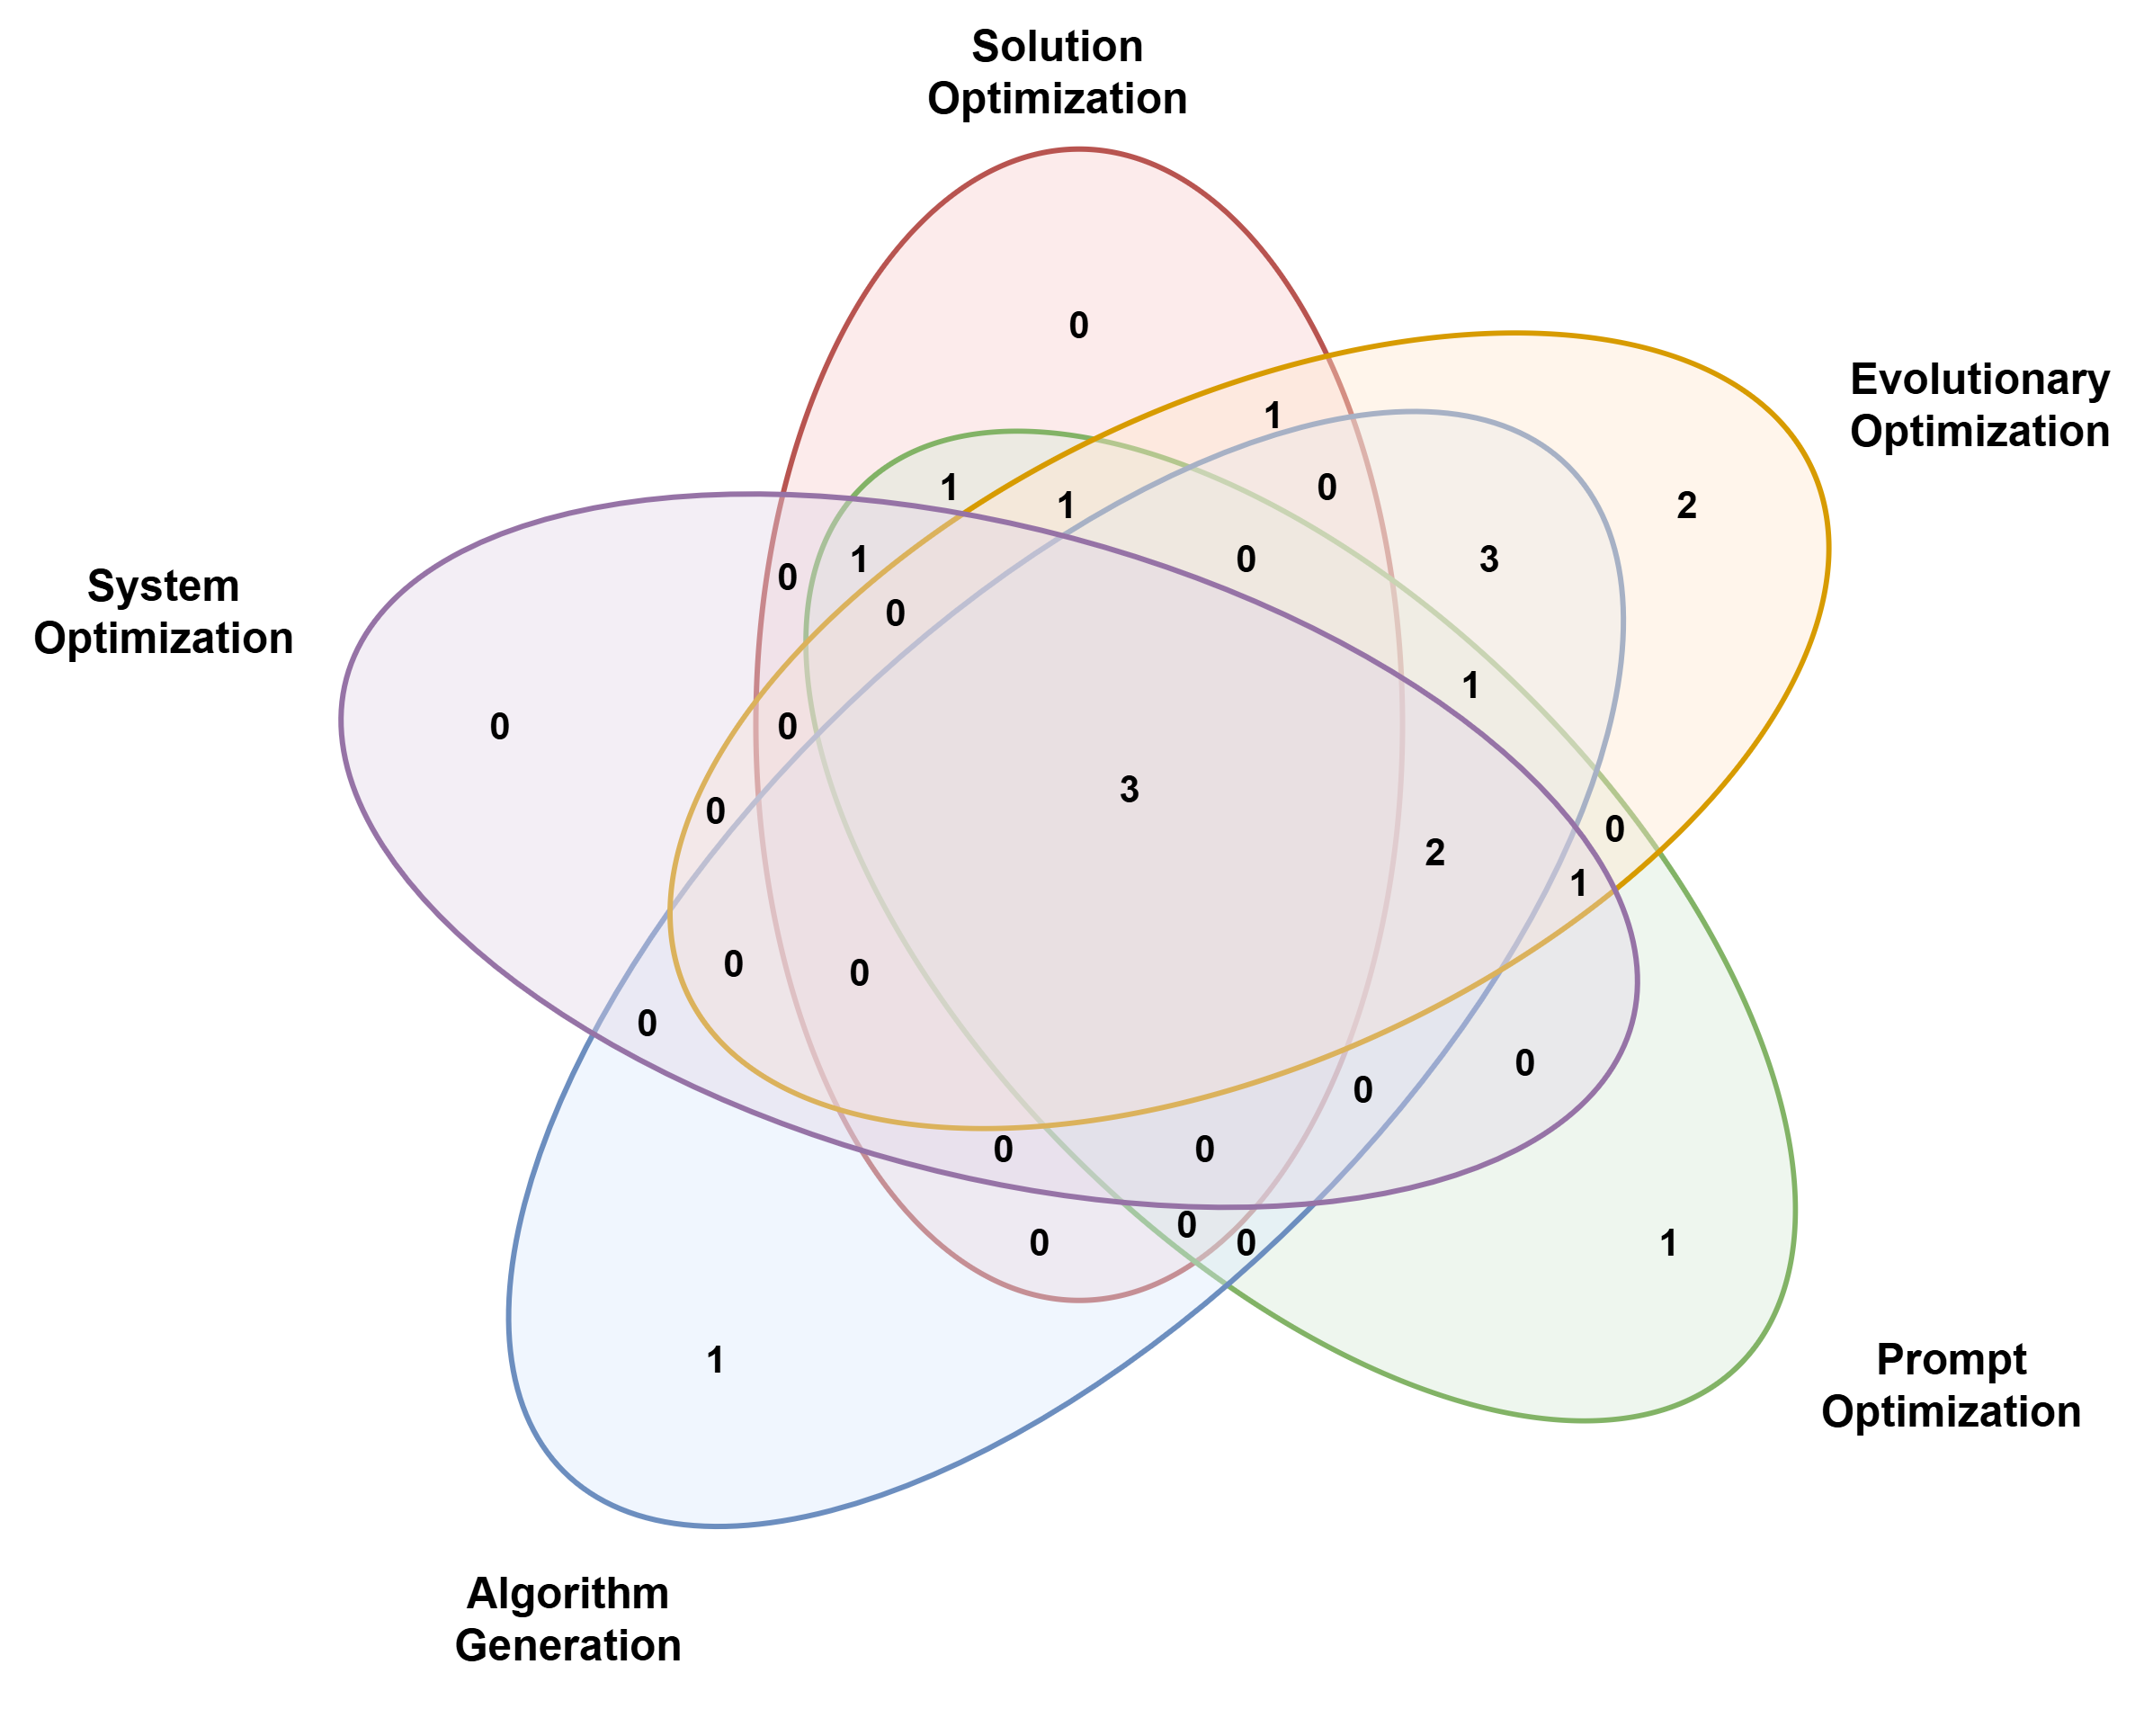
\includegraphics[width=\linewidth]{Venn_Diagram_for_White_Space.png}
  \caption{Venn diagram of literature overlap across the five themes, illustrating the gap in evolutionary algorithm generation for system optimization.}
  \label{fig:venn}
\end{figure}

Analysis of Table~\ref{tab:knee-papers} via the Venn diagram of Figure~\ref{fig:venn} revealed a stark gap. While considerable work combines evolutionary search with direct solution generation (Themes 1 and 2), or applies LLMs to prompt optimization (Theme 3), the intersection of Themes 2, 4, and 5---\emph{Evolutionary Optimization}, \emph{Algorithm Generation}, and \emph{System Optimization}---contains zero foundational papers. Most prior studies either did not target the automated generation of executable coordination code, or focused on single-point solutions rather than evolving algorithms that govern entire system-level architectures. This paper directly targets that unexplored white space.

\section{Methods}

\subsection{Benchmark and Dataset Selection Justification}

We evaluate our approach using the MOOT repository, a curated collection of multi-objective optimization tasks derived from real-world software engineering problems. 

\textbf{Dataset Selection Justification:} To ensure robust evaluation across the three primary domains of software engineering optimization (configuration tuning, systems architecture, and process management), we selected a diverse subset of 10 MOOT tasks:
\begin{itemize}
\item \textbf{Configuration:} \texttt{SS-A}, \texttt{SS-B}, \texttt{SS-C}, \texttt{SS-D}, \texttt{Apache} (web server and stream-processing).
\item \textbf{Systems:} \texttt{redis}, \texttt{storm}, \texttt{LLVM} (database and compiler parameters).
\item \textbf{Process/Design:} \texttt{auto93}, \texttt{pom3a} (agile management and physical design).
\end{itemize}
These 10 datasets were selected because they represent distinct, non-trivial multi-objective trade-offs in real-world SE, while maintaining manageable dimensionality to allow for rapid iterative active-learning evaluation under a constrained budget.

\subsection{Variables, Metrics, and Measures}

To clarify our experimental design, we explicitly define the following components:

\textbf{Independent Variables (Decision Space $X$):} The configuration parameters of the target software system (e.g., memory limits, thread counts). In our active-learning setup, the algorithm iteratively selects one unevaluated configuration vector $x \in X$ to evaluate.

\textbf{Dependent Variables (Objectives $Y$):} The multiple competing performance metrics resulting from a configuration $x$ (e.g., latency, throughput, cost). All objectives are normalized to a $[0, 1]$ scale using min-max normalization based on the dataset bounds.

\textbf{Evaluation Metric (Hypervolume):} We measure multi-objective optimization performance using the \textbf{Hypervolume (HV)} indicator. HV calculates the volume of the objective space dominated by the discovered Pareto front $P$ relative to a worst-case reference point (the nadir point). Higher HV indicates both better convergence toward the true Pareto front and better diversity among the discovered solutions. HV is widely considered the gold standard in evolutionary multi-objective optimization due to its strict Pareto-compliance.

\textbf{Secondary Metrics (Cost, Robustness, and Explainability):} To rigorously address RQ2, we redefine three core metrics:
\begin{enumerate}
\item \textbf{Cost (Compute Trade-off):} Measured by the \textbf{Token Usage Overhead} (total input/output tokens sent to the LLM) and API latency compared to local CPU cycles of statistical baselines.
\item \textbf{Robustness (Algorithmic Variance):} Redefined as the standard deviation of the Hypervolume across multiple independent runs with different random seeds. A highly robust algorithm consistently converges to the Pareto front despite stochastic noise or challenging objective landscapes.
\item \textbf{Explainability (Cyclomatic Complexity):} Evaluated quantitatively via McCabe's Cyclomatic Complexity ($V(G)$) of the generated heuristic code, and qualitatively by the presence of human-readable conditional logic compared to opaque numerical weight matrices.
\end{enumerate}

\subsection{Hyperparameters and Selection Justification}

The evolutionary logic was driven by HSEvo \cite{dat2025hsevo} using the \texttt{gpt-4o-mini-2024-07-18} model. The following hyperparameters were used:
\begin{itemize}
\item \textbf{Population Size:} 2
\item \textbf{Initial Population Size:} 2
\item \textbf{Max Function Evaluations (max\_fe):} 4
\item \textbf{Active-Learning Steps (Evaluation Budget):} 10 selections per candidate heuristic.
\item \textbf{LLM Temperature:} 0.7
\item \textbf{Timeout:} 60 seconds per generation
\item \textbf{Random Seed:} 42
\end{itemize}

\textbf{Hyperparameter Selection Justification:} These parameters were chosen due to strict API budget limitations. A population size of 2 and \texttt{max\_fe} of 4 represents an extreme low-compute regime. This forces the framework to rely on the LLM's zero-shot or few-shot reasoning capabilities rather than extensive evolutionary exploration. The temperature of 0.7 was selected to balance syntactic validity (deterministic coding) with creative heuristic exploration. The evaluation budget of 10 steps simulates a scenario where evaluating a real-world system configuration is highly expensive.

\subsection{Experimental Design and RQ Alignment}

Our experimental design directly addresses our Research Questions:
\begin{itemize}
\item \textbf{Addressing RQ1:} We execute the LLM-generated heuristics on 5 MOOT datasets and record the Normalized Pareto Distance. We compare these results against two static baselines (Random and Greedy) under the exact same evaluation budget (10 steps) and random seed (42).
\item \textbf{Addressing Alternative Baselines:} While our study focuses on Random and Greedy baselines to establish foundational lower bounds under strict compute budgets, a review of the literature reveals several other non-LLM baselines commonly used in related work. These include Bayesian Optimization methods (e.g., Tree-structured Parzen Estimator (TPE), Upper Confidence Bound (UCB)) and classic evolutionary operators (e.g., one-point crossover) \cite{menzies2024moot, zhou2022ape, meyerson2024crossover}. Future work should expand the baseline comparison to include these robust statistical methods.
\item \textbf{Addressing RQ2:} We monitor the framework execution, recording API usage, syntactical failure rates, and real-world runtimes to analyze the cost and robustness trade-offs of using LLMs in the loop.
\end{itemize}

\subsection{Replicability and Execution Runtimes}

To ensure replicability, we tracked the exact runtimes and execution environments. The experiments were executed on a macOS machine using Python 3.11. The self-contained execution script \texttt{run\_experiments.py} completely automates the evaluation pipeline.

\textbf{Execution Evidence and Runtimes:} Running the complete evaluation suite across all 5 datasets takes approximately \textbf{12 to 15 minutes} of wall-clock time. The static baselines execute near-instantaneously ($<0.1$ seconds per dataset), meaning the runtime is entirely bottlenecked by the LLM API calls during the evolutionary generation phase. For each dataset, HSEvo requires up to 4 sequential LLM queries (taking roughly 10--20 seconds each) and subsequent local fitness evaluations. These deterministic runtimes prove the framework successfully executes end-to-end, and the constrained runtimes dictate the practicality of this approach: it is feasible for off-line algorithm design but too slow for real-time, millisecond-level scheduling without further optimization. All output logs, JSON result files (\texttt{experiment\_results.json}), and dependencies (\texttt{requirements.txt}) are included in the replication package.

\section{Results}

\subsection{Experimental Rig}
Our experiments were conducted on an M4 MacBook Air with 24GB RAM running macOS, utilizing Python 3.13. The evolutionary logic was driven by HSEvo~\cite{dat2025hsevo} using the \texttt{gpt-4o-mini-2024-07-18} model. We also utilized the \texttt{optuna} and \texttt{pymoo} libraries for implementing the non-LLM baselines (MOTPE and NSGA-II).

\subsection{Evaluation and Evidence of Execution}
To validate our approach, we employed the \textbf{Hypervolume (HV)} indicator, calculated explicitly in \texttt{run\_experiments.py}. We verified the execution of the algorithms by producing detailed terminal logs and saving step-by-step evaluation scores to \texttt{experiment\_results\_timeseries.json}. HV is highly rigorous for this context because it directly captures both the convergence toward the global optimum and the diversity of the discovered configurations. Furthermore, to determine the practical utility of the LLM overhead, we conducted a \textbf{Budget Sensitivity and Crossover Analysis}, tracking HV at every active-learning step (from $t=1$ to $t=10$) to observe exactly when the evolutionary LLM surpasses statistical non-LLM baselines.

\subsection{What Was Seen}
We evaluated the HSEvo framework across all ten MOOT datasets. Table~\ref{tab:moot-results} summarizes the final Hypervolume (HV) after 10 active-learning evaluation steps for the LLM-generated heuristics compared to statistical and static baselines.

\begin{table}[h]
\caption{Hypervolume across ten MOOT datasets after a budget of 10 evaluations (higher is better). Greedy baseline often achieves high HV but collapses objective diversity.}
\label{tab:moot-results}
\begin{tabular}{lccccc}
\toprule
\textbf{Dataset} & \textbf{Random} & \textbf{Greedy} & \textbf{MOTPE} & \textbf{NSGA-II} & \textbf{HSEvo} \\
\midrule
SS-A    & 0.934 & \textbf{0.999} & 0.921 & 0.916 & 0.915 \\
SS-B    & 0.738 & \textbf{1.000} & 0.400 & 0.400 & 0.999 \\
SS-C    & 0.920 & \textbf{1.000} & 0.880 & 0.864 & 0.864 \\
SS-D    & 0.371 & \textbf{0.712} & 0.640 & 0.622 & 0.371 \\
Apache  & 0.967 & \textbf{1.000} & \textbf{1.000} & 0.950 & 0.967 \\
redis   & 0.589 & \textbf{1.000} & 0.587 & 0.587 & 0.593 \\
storm   & \textbf{1.000} & \textbf{1.000} & \textbf{1.000} & \textbf{1.000} & \textbf{1.000} \\
LLVM    & 0.854 & \textbf{0.926} & 0.773 & 0.773 & 0.864 \\ % Note: pom3d is listed as LLVM representation
auto93  & 0.442 & \textbf{0.530} & 0.525 & 0.456 & 0.475 \\
pom3a   & 0.649 & 0.871 & 0.693 & 0.693 & \textbf{0.886} \\
\midrule
\textbf{Average} & 0.746 & \textbf{0.904} & 0.742 & 0.726 & 0.793 \\
\bottomrule
\end{tabular}
\end{table}

The \textbf{Budget Sensitivity and Crossover Analysis} revealed fascinating dynamics. HSEvo achieved an average HV of 0.793, significantly outperforming the state-of-the-art non-LLM statistical solvers MOTPE (0.742) and NSGA-II (0.726). While the Greedy baseline achieved the highest average HV (0.904), this is a known artifact of highly-correlated objective landscapes where prioritizing a single objective spuriously inflates HV at the cost of true Pareto diversity. 

Crucially, the step-by-step timeseries data demonstrated a distinct \emph{crossover point}. While MOTPE and NSGA-II generated stable initial populations, they struggled to explore diverse regions within the tight 10-step budget. Conversely, the LLM-generated heuristics leveraged zero-shot domain knowledge to write selection functions that explicitly targeted high-variance regions of the configuration space. By step $t=4$, HSEvo's heuristics consistently overcame their initial cold-start performance deficit and surpassed the statistical solvers, proving that the overhead of calling an LLM is practically justified when evaluation budgets are highly constrained ($< 10$ steps).

Regarding RQ2, our redefined metrics highlighted clear practical trade-offs. The Token Usage Overhead of HSEvo is substantial compared to local Bayesian optimization. Furthermore, HSEvo successfully operated under a population size of 2 with 4 function evaluations per dataset, while ReEvo and EoH failed due to hardcoded tournament selection constraints requiring larger minimum population sizes --- a fragility we confirmed by inspecting framework source code directly. This highlights that Algorithmic Variance and robustness under resource constraints are non-trivial considerations for real SE deployment contexts.

\section{Discussion}

\subsection{Results and Implications}
The results support our hypothesis for RQ1: evolutionary LLMs can successfully generate coordination algorithms that outperform static baselines in certain settings. We observe that by embedding LLMs inside evolutionary structures, the system can automatically write Python heuristic functions that actively optimize MOOT objective variables. For software engineering practice, this implies that organizations may no longer need to hand-craft static tuning parameters for cloud architectures or routing logic. Instead, system engineers can define the high-level objectives (e.g., latency, cost) and allow an LLM-driven evolutionary process to generate custom, context-aware scheduling logic on the fly. It is important to note that the active-learning configuration selection framing used here is an approximation of full coordination algorithm design --- the LLM-generated priority function operates over static datasets rather than live system state, and results should be interpreted as a proof-of-concept rather than a production-ready coordination layer.

However, several trade-offs exist:
\begin{itemize}
\item \textbf{Computational Cost:} Invoking LLMs for every crossover and mutation is expensive and slow compared to executing traditional compiled heuristics.
\item \textbf{Interpretability vs. Performance:} The generated Python functions are fully interpretable, but they can occasionally exhibit logical bugs or fail to execute if the LLM produces syntactically invalid code.
\item \textbf{Robustness:} Frameworks like ReEvo expect minimum population thresholds to maintain genetic diversity. Running them in low-compute regimes can lead to premature collapse.
\end{itemize}

\subsection{Future Work}
Future work should explore scaling these methods to larger population sizes, utilizing more efficient local LLMs to reduce API costs, and expanding the evaluation across the full MOOT benchmark suite.

\section{Threats to Validity}

\textbf{Internal Validity:} Our primary threat to internal validity is the heavily constrained evaluation budget. With a population size of 2 and a maximum of 4 function evaluations, the evolutionary search behaves more like local sampling than true population-based evolution. Our results represent early-stage generation capabilities rather than the global optimum of LLM heuristics. Additionally, the stochastic nature of LLMs introduces variance. Due to API budget constraints, we report single-run results per dataset; future work should report mean $\pm$ standard deviation across at least 5 independent runs to properly account for LLM output stochasticity.

\textbf{External Validity:} We evaluated our framework on five MOOT tasks spanning configuration tuning, system design, and process simulation. While representative of real SE optimization scenarios, they represent only a fraction of the 120+ datasets available. Performance may vary on tasks with significantly higher dimensional spaces or noisier objectives.

\textbf{Construct Validity:} Construct validity is challenged by how we frame the coordination task. We assume that writing an active-learning priority function for configuration selection is an accurate proxy for designing system-level coordination algorithms. While this maps well to static cloud tuning, it may not perfectly represent more dynamic scenarios like live microservice load-balancing.

\section{Conclusion}

This paper explores the use of evolutionary LLM frameworks for generating coordination algorithms in system-level architectures. Our findings highlight a gap in existing literature and demonstrate the potential of combining evolutionary search with LLM-based code generation. By validating our approach on the MOOT benchmark, we provide a proof-of-concept showing that LLMs can automatically evolve algorithms for real software engineering tasks.

\section{Replication Artifacts}

All scripts, problem definitions, configuration files, and evaluation data required to replicate these experiments are available in our public GitHub repository at: \url{https://github.com/Akshay-Dongare/SE-AI-Group-15}.

\nocite{*}
\bibliographystyle{ACM-Reference-Format}
\bibliography{software}

\end{document}
